

%%
% ein bild mit rechter caption
%%%%%%%%%%%%%%%%%%%%%%%%%%%%%%%%%%%%%%%%%%%%%%%%%%%%
\begin{SCfigure}
  \centering
  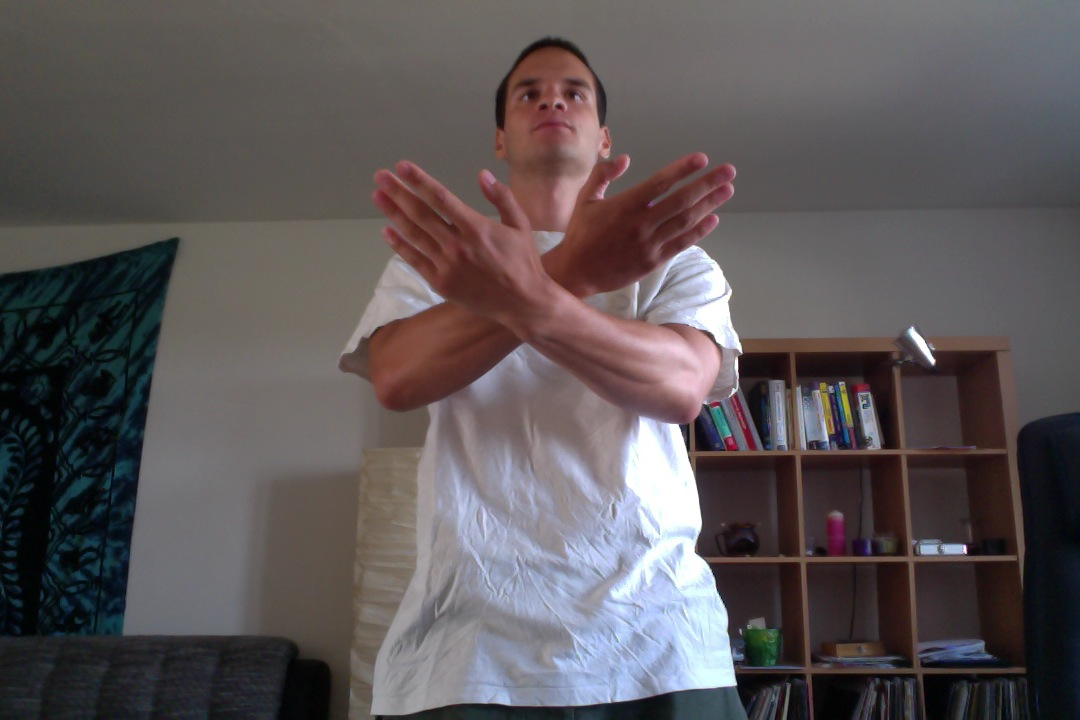
\includegraphics[width=0.5\textwidth]
    {resources/images/siunimtau/1/1}
  \caption{ ... caption text ... }
\end{SCfigure}




%%
% ein bild horizontal flippen 
%%%%%%%%%%%%%%%%%%%%%%%%%%%%%%%%%%%%%%%%%%%%%%%%%%%%
\begin{figure}[h!]
  \centering
    \reflectbox{%
      \includegraphics[width=0.5\textwidth]{gull}}
  \caption{A picture of the same gull
           looking the other way!}
\end{figure}





%%
% sidecaptions
%%%%%%%%%%%%%%%%%%%%%%%%%%%%%%%%%%%%%%%%%%%%%%%%%%%%
============================ [https://en.wikibooks.org/wiki/LaTeX/Floats,_Figures_and_Captions]
It is sometimes desirable to have a caption appear on the side of a float, rather than above or below. The sidecap package can be used to place a caption beside a figure or table. The following example demonstrates this for a figure by using a SCfigure environment in place of the figure environment.
- Wrapping text around figures

!! Subfloats von \usepackage{subcaption}
	\begin{figure}
	        \begin{subfigure}[b]{0.3\textwidth}







%%
% Multiple indices
%%%%%%%%%%%%%%%%%%%%%%%%%%%%%%%%%%%%%%%%%%%%%%%%%%%%
\usepackage{multind}
\makeindex{books}
\makeindex{authors}
...
\index{books}{A book to index}
\index{authors}{Put this author in the index}
...
\printindex{books}{The Books index}
\printindex{authors}{The Authors index}


\usepackage{multicol,multind}

\makeatletter
\def\number@of@cols{2}
\renewcommand{\printindex}[3][2]{%
  \section*{#3}%
  \@mkboth{\MakeUppercase{#3}}{\MakeUppercase{#3}}%
  \addcontentsline{toc}{section}{#3}%
  \parindent\z@ \def\number@of@cols{#1}%
  \@input{#2.ind}%
}
\renewenvironment{theindex}
  {\begin{multicols}{\number@of@cols}
   \parskip\z@ \@plus .3\p@\relax
   \columnseprule \z@
   \columnsep 35\p@
   \let\item\@idxitem}
  {\end{multicols}}
\makeatother

\makeindex{indexa}
\makeindex{indexb}





%%
% bibliography
%%%%%%%%%%%%%%%%%%%%%%%%%%%%%%%%%%%%%%%%%%%%%%%%%%%%

%\bibliographystyle{plain}%alpha
%\bibliography{includes/bibliography}


%\begin{thebibliography}{widest entry}
%\bibitem[label1]{cite_key1} bibliographic information \bibitem[label2]{cite_key2} %bibliographic information
%... \end{thebibliography}

\begin{thebibliography}{9}

\bibitem{lamport94}
  Leslie Lamport,
  \emph{\LaTeX: A Document Preparation System}.
  Addison Wesley, Massachusetts,
  2nd Edition,
  1994.

\end{thebibliography}




@book{lamport94,
    author    = "Michel Goossens and Frank Mittlebach and Alexander Samarin",
    title     = "The Latex Companion",
    year      = "1993",
    publisher = "Addison-Wesley",
    address   = "Reading, Massachusetts"
}
